\documentclass[12pt]{article}
\usepackage{amsmath, amsfonts, mathtools, amsthm, amssymb}
\usepackage{geometry}
\usepackage{float}
\usepackage{mathrsfs}
\usepackage{booktabs}
\usepackage{mathtools}
\usepackage{enumerate}
\usepackage{graphicx}
\usepackage{indentfirst}
\usepackage[dvipsnames]{xcolor}
\usepackage{color}
\usepackage{caption}
\usepackage{array}
\usepackage{etoolbox}
\usepackage{physics}
\usepackage{siunitx}
\usepackage[natbib=true,style=numeric,sorting=none]{biblatex}
\usepackage[T1]{fontenc}
\usepackage{inconsolata}
\usepackage[nodayofweek]{datetime}
\usepackage[british]{datetime2}
\usepackage{lastpage}
\usepackage[colorlinks=true,linkcolor=blue,urlcolor=red]{hyperref}
% quiver style
\usepackage{tikz-cd}
% `calc` is necessary to draw curved arrows.
\usetikzlibrary{calc}
% `pathmorphing` is necessary to draw squiggly arrows.
\usetikzlibrary{decorations.pathmorphing}

% A TikZ style for curved arrows of a fixed height, due to AndréC.
\tikzset{curve/.style={settings={#1},to path={(\tikztostart)
					.. controls ($(\tikztostart)!\pv{pos}!(\tikztotarget)!\pv{height}!270:(\tikztotarget)$)
					and ($(\tikztostart)!1-\pv{pos}!(\tikztotarget)!\pv{height}!270:(\tikztotarget)$)
					.. (\tikztotarget)\tikztonodes}},
	settings/.code={\tikzset{quiver/.cd,#1}
			\def\pv##1{\pgfkeysvalueof{/tikz/quiver/##1}}},
	quiver/.cd,pos/.initial=0.35,height/.initial=0}

% TikZ arrowhead/tail styles.
\tikzset{tail reversed/.code={\pgfsetarrowsstart{tikzcd to}}}
\tikzset{2tail/.code={\pgfsetarrowsstart{Implies[reversed]}}}
\tikzset{2tail reversed/.code={\pgfsetarrowsstart{Implies}}}
% TikZ arrow styles.
\tikzset{no body/.style={/tikz/dash pattern=on 0 off 1mm}}

% useful macro for class
\newcommand{\probability}[2]{\mathbb{\MakeUppercase{P}}_{#1} \left(#2\right)}
\newcommand{\variance}[2]{\mathrm{Var}_{#1} \left[ #2 \right]}
\newcommand{\expectation}[2]{\mathbb{\MakeUppercase{E}}_{#1} \left[#2\right]}
\newcommand{\at}[3]{\left.#1\right\vert_{#2}^{#3}}
\newcommand\quotient[2]{
	\mathchoice
	{% \displaystyle
		\text{\raise1ex\hbox{$#1$}\Big/\lower1ex\hbox{$#2$}}%
	}
	{% \textstyle
		#1\,/\,#2
	}
	{% \scriptstyle
		#1\,/\,#2
	}
	{% \scriptscriptstyle  
		#1\,/\,#2
	}
}
\newcommand{\identity}{\mathrm{id}}
\newcommand{\sinc}{\mathop{\mathrm{sinc}}}
\newcommand{\rect}{\mathop{\mathrm{rect}}}
\newcommand{\tri}{\mathop{\mathrm{tri}}}
\newcommand{\Real}{\mathop{\mathrm{Re}}}

\newcommand{\Homomorphism}{\mathrm{Hom}}
\newcommand{\Morphism}{\mathrm{Mor}}
\newcommand{\Object}{\mathrm{Ob}}

\usepackage{physics}

\DeclareMathOperator{\im}{Im}
\DeclareMathOperator{\sgn}{sgn}
\DeclareMathOperator{\Int}{Int}
\DeclareMathOperator{\diag}{diag}

\let\implies\Rightarrow
\let\impliedby\Leftarrow
\let\iff\Leftrightarrow

\usepackage{stmaryrd} % for \lightning
\newcommand\conta{\scalebox{1.1}{\(\lightning\)}}

\usepackage{bm}
\usepackage{bbm}


% figure support
\usepackage{import}
\usepackage{xifthen}
\pdfminorversion=7
\usepackage{pdfpages}
\usepackage{transparent}
\newcommand{\incfig}[1]{%
	\def\svgwidth{\columnwidth}
	\import{./picture/}{#1.pdf_tex}
}


% when you need multi-row in tabular
\usepackage{multirow}

\geometry{a4paper,left=2.54cm,right=2.54cm,top=2.54cm,bottom=2.54cm}
\setlength{\headheight}{13.59999pt}
\setlength{\parindent}{1em}
\thispagestyle{empty}

\newcolumntype{P}[1]{>{\centering\arraybackslash}p{#1}}
\renewcommand{\qed}{\hfill\(\blacksquare\)}

\renewcommand{\emph}[1]{{\color{Turquoise3}\textsl{#1}}}
\definecolor{Turquoise3}{RGB}{0, 134, 139}

\newcommand\blfootnote[1]{%
	\begingroup
	\renewcommand\thefootnote{}\footnote{#1}%
	\addtocounter{footnote}{-1}%
	\endgroup
}

% horizontal rule
\newcommand\hr{
	\noindent\rule[0.5ex]{\linewidth}{0.5pt}
}

% TodoNotes and inline notes in fancy boxes
\usepackage{todonotes}
\usepackage{tcolorbox}

% Algorithm Env
\usepackage[linesnumbered,lined,vlined,ruled,commentsnumbered]{algorithm2e}
\SetKwComment{Comment}{// }{}
\SetArgSty{textsl}

\pdfsuppresswarningpagegroup=1
\usepackage{fancyhdr} % Required for customizing headers and footers

\pagestyle{fancy} % Enable custom headers and footers

\lhead{\small\Instuition: \   \Course} % Left header; output the instructor in brackets if one was set
\chead{} % Centre header
\rhead{}

\rhead{\small\ifdef{\DueDate}{Due\ \DueDate}{}} % Right header; output the author name if one was set, otherwise the due date if that was set


\lfoot{} % Left footer
\cfoot{\small Page\ \thepage\ of\ \pageref{LastPage}} % Centre footer
\rfoot{} % Right footer

% Appendix environment
\usepackage{appendix}
\def\sectionautorefname{Section}
\def\subsectionautorefname{Section}
\def\appendixautorefname{Appendix}
\renewcommand\appendixname{Appendix}
\renewcommand\appendixtocname{Appendix}
\renewcommand\appendixpagename{Appendix}
% begin appendix autoref patch [\autoref subsections in appendix](https://tex.stackexchange.com/questions/149807/autoref-subsections-in-appendix)
\makeatletter
\patchcmd{\hyper@makecurrent}{%
	\ifx\Hy@param\Hy@chapterstring
		\let\Hy@param\Hy@chapapp
	\fi
}{%
	\iftoggle{inappendix}{%true-branch
		% list the names of all sectioning counters here
		\@checkappendixparam{chapter}%
		\@checkappendixparam{section}%
		\@checkappendixparam{subsection}%
		\@checkappendixparam{subsubsection}%
		\@checkappendixparam{paragraph}%
		\@checkappendixparam{subparagraph}%
	}{}%
}{}{\errmessage{failed to patch}}

\newcommand*{\@checkappendixparam}[1]{%
	\def\@checkappendixparamtmp{#1}%
	\ifx\Hy@param\@checkappendixparamtmp
		\let\Hy@param\Hy@appendixstring
	\fi
}
\makeatletter

\newtoggle{inappendix}
\togglefalse{inappendix}

\apptocmd{\appendix}{\toggletrue{inappendix}}{}{\errmessage{failed to patch}}
\apptocmd{\subappendices}{\toggletrue{inappendix}}{}{\errmessage{failed to patch}}
% end appendix autoref patch

% Environments
\makeatother
% For box around Definition, Theorem, etc.
\usepackage{mdframed}
\mdfsetup{skipabove=1em,skipbelow=0em}
\theoremstyle{definition}
\newmdtheoremenv[nobreak=true]{definition}{Definition}[section]
\providecommand*\definitionautorefname{Definition}
\newmdtheoremenv[nobreak=true]{theorem}{Theorem}[section]
\providecommand*\theoremautorefname{Theorem}
\newmdtheoremenv[nobreak=true]{lemma}{Lemma}[section]
\providecommand*\lemmaautorefname{Lemma}
\newmdtheoremenv[nobreak=true]{corollary}{Corollary}[section]
\providecommand*\corollaryautorefname{Corollary}
\newmdtheoremenv[nobreak=true]{proposition}{Proposition}[section]
\providecommand*\propositionautorefname{Proposition}

\makeatletter

\renewcommand\headrulewidth{0.5pt}

\makeatletter
\def\@maketitle{%
	\newpage
	\null
	\vskip 2em%
	\begin{center}%
		\let \footnote \thanks
		{\LARGE \@title \par}%
		\vskip 1.5em%
			{\large
				\lineskip .5em%
				\begin{tabular}[t]{c}%
					\@author \\
                    \ifdef{\Instructor}{Instructor:\\ \Instructor}{}
					\normalsize{
						\ifdef{\Uniquname}{Uniquname: \Uniquname}{}
						\hspace{1em}
						\ifdef{\UMID}{umid: \UMID}{}
					}
				\end{tabular}\par}%
		\vskip 1em%
			{\large \@date}%
	\end{center}%
	\par
	\vskip 1.5em
}
\makeatother

\title{
	\begin{center}
		\rule{15cm}{0.01cm}
		\\\LARGE{
			\Instuition
			%\\
			%\SeasonYear
			\\
			\Course
		}
		\\\rule{15cm}{0.01cm}
		\\\vspace{6cm}
		\begin{huge}
			\sc{\Title}
		\end{huge}
	\end{center}
	\vfill
	\flushleft
	\ifdef{\Group}{
		\begin{center}
			\large
			\sc{\Group}
			\mbox{}
		\end{center}
	}{}
}

\usepackage{listings}
\usepackage[utf8]{inputenc}
\usepackage[english]{babel}
\definecolor{maroon}{cmyk}{0, 0.87, 0.68, 0.32}
\definecolor{halfgray}{gray}{0.55}
\definecolor{ipython_frame}{RGB}{207, 207, 207}
\definecolor{ipython_bg}{RGB}{247, 247, 247}
\definecolor{ipython_red}{RGB}{186, 33, 33}
\definecolor{ipython_green}{RGB}{0, 128, 0}
\definecolor{ipython_cyan}{RGB}{64, 128, 128}
\definecolor{ipython_purple}{RGB}{170, 34, 255}

\colorlet{mygray}{black!30}
\colorlet{mygreen}{green!60!blue}
\colorlet{mymauve}{red!60!blue}
\lstdefinelanguage{commandline}{
	basicstyle=\ttfamily,
	columns=fullflexible,
	breakatwhitespace=false,
	breaklines=true,
	captionpos=b,
	commentstyle=\color{mygreen},
	extendedchars=true,
	frame=single,
	keepspaces=true,
	keywordstyle=\color{blue},
	language=c++,
	numbers=none,
	numbersep=5pt,
	numberstyle=\tiny\color{blue},
	rulecolor=\color{mygray},
	showspaces=false,
	showtabs=false,
	stepnumber=5,
	stringstyle=\color{mymauve},
	tabsize=3,
	title=\lstname
}
\lstset{
breaklines=true,
%
extendedchars=true,
literate=
	{á}{{\'a}}1 {é}{{\'e}}1 {í}{{\'i}}1 {ó}{{\'o}}1 {ú}{{\'u}}1
{Á}{{\'A}}1 {É}{{\'E}}1 {Í}{{\'I}}1 {Ó}{{\'O}}1 {Ú}{{\'U}}1
{à}{{\`a}}1 {è}{{\`e}}1 {ì}{{\`i}}1 {ò}{{\`o}}1 {ù}{{\`u}}1
{À}{{\`A}}1 {È}{{\'E}}1 {Ì}{{\`I}}1 {Ò}{{\`O}}1 {Ù}{{\`U}}1
{ä}{{\"a}}1 {ë}{{\"e}}1 {ï}{{\"i}}1 {ö}{{\"o}}1 {ü}{{\"u}}1
{Ä}{{\"A}}1 {Ë}{{\"E}}1 {Ï}{{\"I}}1 {Ö}{{\"O}}1 {Ü}{{\"U}}1
{â}{{\^a}}1 {ê}{{\^e}}1 {î}{{\^i}}1 {ô}{{\^o}}1 {û}{{\^u}}1
{Â}{{\^A}}1 {Ê}{{\^E}}1 {Î}{{\^I}}1 {Ô}{{\^O}}1 {Û}{{\^U}}1
{œ}{{\oe}}1 {Œ}{{\OE}}1 {æ}{{\ae}}1 {Æ}{{\AE}}1 {ß}{{\ss}}1
{ç}{{\c c}}1 {Ç}{{\c C}}1 {ø}{{\o}}1 {å}{{\r a}}1 {Å}{{\r A}}1
{€}{{\EUR}}1 {£}{{\pounds}}1
}

%%
%% Python definition (c) 1998 Michael Weber
%% Additional definitions (2013) Alexis Dimitriadis
%% modified by me (should not have empty lines)
%%
\lstdefinelanguage{iPython}{
morekeywords={access,and,break,class,continue,def,del,elif,else,except,exec,finally,for,from,global,if,import,in,is,lambda,not,or,pass,print,raise,return,try,while},%
%
% Built-ins
morekeywords=[2]{abs,all,any,basestring,bin,bool,bytearray,callable,chr,classmethod,cmp,compile,complex,delattr,dict,dir,divmod,enumerate,eval,execfile,file,filter,float,format,frozenset,getattr,globals,hasattr,hash,help,hex,id,input,int,isinstance,issubclass,iter,len,list,locals,long,map,max,memoryview,min,next,object,oct,open,ord,pow,property,range,raw_input,reduce,reload,repr,reversed,round,set,setattr,slice,sorted,staticmethod,str,sum,super,tuple,type,unichr,unicode,vars,xrange,zip,apply,buffer,coerce,intern},%
%
sensitive=true,%
morecomment=[l]\#,%
morestring=[b]',%
morestring=[b]",%
%
morestring=[s]{'''}{'''},% used for documentation text (mulitiline strings)
morestring=[s]{"""}{"""},% added by Philipp Matthias Hahn
%
morestring=[s]{r'}{'},% `raw' strings
morestring=[s]{r"}{"},%
morestring=[s]{r'''}{'''},%
morestring=[s]{r"""}{"""},%
morestring=[s]{u'}{'},% unicode strings
morestring=[s]{u"}{"},%
morestring=[s]{u'''}{'''},%
morestring=[s]{u"""}{"""},%
%
% {replace}{replacement}{lenght of replace}
% *{-}{-}{1} will not replace in comments and so on
literate=
	{á}{{\'a}}1 {é}{{\'e}}1 {í}{{\'i}}1 {ó}{{\'o}}1 {ú}{{\'u}}1
{Á}{{\'A}}1 {É}{{\'E}}1 {Í}{{\'I}}1 {Ó}{{\'O}}1 {Ú}{{\'U}}1
{à}{{\`a}}1 {è}{{\`e}}1 {ì}{{\`i}}1 {ò}{{\`o}}1 {ù}{{\`u}}1
{À}{{\`A}}1 {È}{{\'E}}1 {Ì}{{\`I}}1 {Ò}{{\`O}}1 {Ù}{{\`U}}1
{ä}{{\"a}}1 {ë}{{\"e}}1 {ï}{{\"i}}1 {ö}{{\"o}}1 {ü}{{\"u}}1
{Ä}{{\"A}}1 {Ë}{{\"E}}1 {Ï}{{\"I}}1 {Ö}{{\"O}}1 {Ü}{{\"U}}1
{â}{{\^a}}1 {ê}{{\^e}}1 {î}{{\^i}}1 {ô}{{\^o}}1 {û}{{\^u}}1
{Â}{{\^A}}1 {Ê}{{\^E}}1 {Î}{{\^I}}1 {Ô}{{\^O}}1 {Û}{{\^U}}1
{œ}{{\oe}}1 {Œ}{{\OE}}1 {æ}{{\ae}}1 {Æ}{{\AE}}1 {ß}{{\ss}}1
{ç}{{\c c}}1 {Ç}{{\c C}}1 {ø}{{\o}}1 {å}{{\r a}}1 {Å}{{\r A}}1
{€}{{\EUR}}1 {£}{{\pounds}}1
%
{^}{{{\color{ipython_purple}\^{}}}}1
{=}{{{\color{ipython_purple}=}}}1
%
{+}{{{\color{ipython_purple}+}}}1
{*}{{{\color{ipython_purple}$^\ast$}}}1
{/}{{{\color{ipython_purple}/}}}1
%
{+=}{{{+=}}}1
{-=}{{{-=}}}1
{*=}{{{$^\ast$=}}}1
{/=}{{{/=}}}1,
literate=
	*{-}{{{\color{ipython_purple}-}}}1
{?}{{{\color{ipython_purple}?}}}1,
%
identifierstyle=\color{black}\ttfamily,
commentstyle=\color{ipython_cyan}\ttfamily,
stringstyle=\color{ipython_red}\ttfamily,
keepspaces=true,
showspaces=false,
showstringspaces=false,
%
rulecolor=\color{ipython_frame},
frame=single,
frameround={t}{t}{t}{t},
framexleftmargin=6mm,
numbers=left,
numberstyle=\tiny\color{halfgray},
%
%
backgroundcolor=\color{ipython_bg},
%   extendedchars=true,
basicstyle=\scriptsize,
keywordstyle=\color{ipython_green}\ttfamily,
}
\lstdefinestyle{DOS}
{
	backgroundcolor=\color{black},
	basicstyle=\scriptsize\color{white}\ttfamily
}
\author{Chia-Cheng, Hao \quad Le-Rong, Hsu \quad Wei-Chieh, Hung \quad TBD \quad TBD \quad TBD}
\newcommand{\Instuition}{2022 NCTS USRP Group 7}
%\newcommand{\SeasonYear}{}
\newcommand{\Course}{Planar Statistical Physics and Bernoulli Percolation}
\newcommand{\Title}{Final Report}
%\newcommand{\Group}{7}
%\newcommand{\Uniquname}{}
%\newcommand{\UMID}{5950 8197}
\newcommand{\Instructor}{Prof. Jhih-Huang Li(NTU), Prof. Wai-Kit Lam(NTU)}
%\newcommand{\DueDate}{\DTMdisplaydate{2021}{9}{27}{-1}}
\newcommand{\sixedge}{\mbox{\parbox[t][-2pt][c]{10pt}{\scriptsize$\blacktriangledown\hspace{-3.6pt}\blacktriangle\hspace{-4pt}\blacktriangledown$}\hspace{-10.2pt}\parbox[b][10.7pt][c]{10pt}{\scriptsize$\blacktriangle\hspace{-3.6pt}\blacktriangledown\hspace{-3.6pt}\blacktriangle$}}}
\usepackage{graphicx}
\theoremstyle{plane}
\newtheorem*{thm}{Theorem}
\newtheorem*{cor}{Corollary}
\newtheorem*{claim}{Claim}
\newtheorem*{prop}{Proposition}
\newtheorem*{application}{Application}
\theoremstyle{definition}
\newtheorem{case}{Case}
\newtheorem*{defn}{Definition}
\newtheorem*{remark}{Remark}

\begin{document}

\clearpage\maketitle
\thispagestyle{empty}

\newpage
\setcounter{page}{1}
%----------------------------------------------------------------------------------------------------------------------------------------------------
\section{Abstract}
We study the percolation phenomenon in planar statistical physics using probability theory tools. We especially focus on \textit{Bernoulli percolation model}. 
In the first three weeks, we received classes covering four main topics. Those classes introduce methods to discuss the connecting property and phase transition behavior on some regular lattice such as $\mathbb{Z}^2,\mathbb{T}_d$, triangular lattice or hexagon lattice. 
After the classes were over, we went on individual research to explore topics such as exponential decay near critical probability and scaling invariant property of the crossing events.

A more detailed version is on our \href{https://github.com/ausernamess/2022USRP-Group-7/blob/main/main.pdf}{Github} page. 

The link to Prof. Li's USRP webpage at \href{https://usrp2022.cadlag.space/}{here}
\section{Course Progress}

\setcounter{subsection}{-1}
\subsection{(Planer) Statistical Mechanics}
Hao is working on this

%----------
\subsection{Planar Statistical Physics and Bernoulli Percolation}
Given an infinite undirected connected graph $G$. We say an edge $e$ is open(resp., closed) if and only if the edge $e$ is assigned the value $1$(resp., $0$). The name "Bernoulli" is given because we put i.i.d. Bernoulli random variables on each edge and each edge opens with probability $p\in[0,1]$. A configuration $\omega$ is an event that each edge $e\in \text{E}(G)$ is either open or closed. Two vertices $a$ and $b$ are connected if there exists a path from $a$ to $b$. A cluster is a set of vertices that every pair of vertices is connected. If a cluster is infinite, then we say that it is an infinite cluster. We define a function $\theta(p)=\mathbb{P}_p(\exists\text{ an infinite cluster containing }0)$, that is, the probability of the event in the parentheses under the Bernoulli percolation with probability $p$. The key ingredient of the Bernoulli percolation is the critical probability \[p_c\coloneqq\\sup\{p\in [0,1]\mid \theta(p)=0\}\] under which the behavior of percolation changes significantly. The focus of our course is the existence and uniqueness of the infinite cluster and the behavior of the percolation when $p>p_c$ and $p<p_c$. 

%----------
\subsection{Useful Identities \& Applications}
We introduce some fundamental tools which are useful when we study the Bernoulli percolation on other graphs. One important idea is the increasing event. Intuitively, if $A$ is an increasing event, $\omega\in A$ and $\omega\leq\omega'$, then $\omega'$ is in $A$. One noteworthy thing is that we usually consider the increasing events that "depend on finitely many edges". This comes our first tool, Harris-FKG inequality.
\begin{thm}
If $A$ and $B$ are two increasing events, then $\mathbb{P}(A\cap B)\geq \mathbb{P}(A)\mathbb{P}(B)$.
\end{thm}
This is equivalent to 
\begin{thm}
If \(f\) and \(g\) are increasing functions, then $\mathbb{E}[fg]\geq\mathbb{E}[f]\mathbb{E}[g].$
\end{thm}
The Harris-FKG inequality can be applied to the proof that on $\mathbb{Z}^2$, $p_c(\mathbb{Z}^2)\geq 1/2$ with the square-root trick. Another important tool is the B.K. inequality.
\begin{thm}
If A and B are increasing events that depend on finitely many edges, we have \[\mathbb{P}(A\circ B)\leq\mathbb{P}(A)\mathbb{P}(B).\]
\end{thm}
The event $A\circ B$ denotes "$A$ and $B$ are realized disjointly". We could view $A\circ B$ as "the edges that $A$ and $B$ depend on are disjoint". The equality holds when the events $A$ and $B$ are disjoint. Intuitively, the B.K. inequality tells us that if an increasing event holds then it gets harder for another increasing event to hold disjointly. We can manage to use this inequality in order to bound the some probability. The last tool is Russo's identity. This is useful when we study of the behavior $\mathbb{P}_p$ when $p$ varies. Here, it's necessary to introduce the idea of 
pivotal edges. An edge $e$ is said to be pivotal of the configuration $\omega$ if the "switch" of $e$ determines whether $\omega$ is in the event $A$ or not. Write $N(A)=N(A,\omega)$ be the number of pivotal edges in $\omega$. 
\begin{prop}
For an increasing event $A$ depending on finitely many edges, we have \[\frac{d}{dp}\mathbb{P}_p (A)=\mathbb{E}_p[N(A)].\]
\end{prop}
The identity is essential for the study of behavior of supercritical regime. 
>>>>>>> ecad8e7a64f7a529bd91aa55c764861710a58540
%----------
\subsection{Exponential Decay}\label{Course_Progress:Exponentia_Decay}
One of the reason we introduce exponential decay is to show that $p_c \leq \frac{1}{2}$ on $\mathbb{Z}^d$(shown by Harry Kesten in the 80s). 
For $\mathbb{Z}^d$ with $d\geq 1$, depending on whether $p$ is larger than $p_c$, the probability of the origin connected to $\partial \Lambda_n$  ($0 \longleftarrow \partial \Lambda_n$) will either decay exponentially as $n$ grows or bounded below by a constant depending on p. 
Once knowing the above fact, we can show that $\mathbb{P}_p (\mathcal{H}_n)$, the probability of horizontal crossing on $R_n$($[0,n]\times [0,n+1]$) box, also decrease exponentially as $n$ grows under $p < p_c$. 
In the discussion of $\mathbb{Z}^2$, if $p_c < \frac{1}{2}$, we will get a contradiction to $\mathbb{P}_{\frac{1}{2}}(\mathcal{H}_n) = 1/2$ for any $n \in \mathbb{N}$. Therefore, combining the previous discussion we know $p_c = \frac{1}{2}$ on $\mathbb{Z}^2$.

We can observe exponential decay on other event. For example, the size of $C$, where $C$ is the connected component containing the origin, and the probability of the origin connected to a point on one axis with distance $n$ ($0 \longleftarrow ne_1$). In the latter event, we applied the extension of Fekete subadditive lemma to get the parameter for the decay, \textit{correlation length} $\xi(p)$. 
Using the same method, the rate of decay $\varphi(p)$ for $0 \longleftarrow \partial \Lambda_n$ is also acquired, and we know $\varphi(p) = \xi(p)^{-1}$.

%----------
\subsection{Russo-Seymour-Welsh Theorem}
In this section, we discuss the scale invariant property of some connecting events when $p=p_c$ on $\mathbb{Z}^2$ lattice. In particular, we presents the invariant behaviour of the \textit{horizontal crossing event in a rectangle of size $[0,\rho n]\times[0,n]$}, which is denoted by $\mathcal{H}(\rho n, n)$.\\ \\
\textbf{Theorem (Russo-Seymour-Welsh).}
\textit{Let $\rho>0$. There exists $c=c(\rho)>0$ such that for all $n\geq 1$, we have}
\begin{equation*}
c\leq\mathbb{P}_{\frac{1}{2}}\big[\mathcal{H}(\rho n, n)\big]\leq 1-c,
\end{equation*}
\textit{where $\mathcal{H}(\rho n, n)$ denotes the horizontal crossing event in a rectangle with size $[0,\rho n]\times [0,n]$.}\\ \\
They proved this theorem by proving a special case:\\
\textbf{Theorem.} \textit{For all }$n\geq 1$,
\begin{equation*}
\mathbb{P}_{\frac{1}{2}}\big[\mathcal{H}(3n,2n)\big]\geq\frac{1}{128}.
\end{equation*}\\
Once one get this result, i.e. when one find $c(\rho)$ for some $\rho>1$ (e.g. $c(3/2)$), then one can get $c(\rho')$ for arbitrary $\rho'>1$ by construct the crossing events $\mathcal{H}(\rho n,n)$ that assures $\mathcal{H}(\rho'n, n)$ to occur, and hence we can prove the first theorem. For example, to get a lower bound for $\mathbb{P}_{p_c}[\mathcal{H}(4n,n)]$, we can place five $(2n,n)$ boxes as follows: Let $R_1=[0,2n]\times[0,n]$, $R_2=[n,2n]\times[-n,n]$, $R_3=[n,3n]\times[-n,0]$, $R_4=[2n,3n]\times[-n,n]$ and $R_5=[2n,4n]\times[0,n]$. Then we have
\begin{equation*}
\mathbb{P}_{p_c}[\mathcal{H}(R_1)\cap\mathcal{V}(R_2)\cap\mathcal{H}(R_3)\cap\mathcal{V}(R_4)\cap\mathcal{H}(R_5)]\leq\mathbb{P}_{p_c}[\mathcal{H}([0,4n]\times[0,n])].
\end{equation*}
Now by Harris-FKG inequality and translation invariant property on $\mathbb{Z}^2$ lattice, we immediately have
\begin{equation*}
c(2)^5\leq \mathbb{P}_{p_c}[\mathcal{H}(4n,n)].
\end{equation*}

With Russo-Seymour-Welsh's theory, we're able to give a scale invariant property for more general crossing events. Consider a simply connected domain with a smooth boundary $\Omega$ with distinct boundary points $a,b,c,d$. For $\delta>0$, we define a finite graph $\Omega^\delta=\delta\mathbb{Z}^2\cap\Omega$. And let $a^\delta, b^\delta, c^\delta, d^\delta\in\Omega^\delta$ to be the closest points to $a,b,c,d\in\partial\Omega$. Also define $(a^\delta b^\delta),\,(c^\delta d^\delta)$ as the paths on $\partial\Omega^\delta$ from $a^\delta$ to $b^\delta$, from $c^\delta$ to $d^\delta$ counterclockwise.\\ \\
\textbf{Theorem.} \textit{There exists $c=c(\Omega,a,b,c,d)>0$ such that for any $\delta>0$,}
\begin{equation*}
\mathbb{P}_\frac{1}{2}\big[(a^\delta b^\delta)\xleftrightarrow{\text{$\Omega^\delta$}}(c^\delta d^\delta)\big]\geq c.
\end{equation*}
    
\begin{figure}[b]
\centering
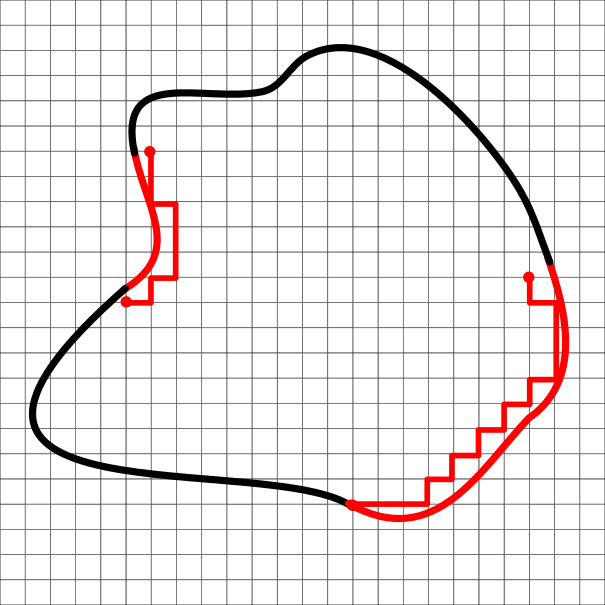
\includegraphics[width=5.0cm]{./RSWpart/omega_2.png}
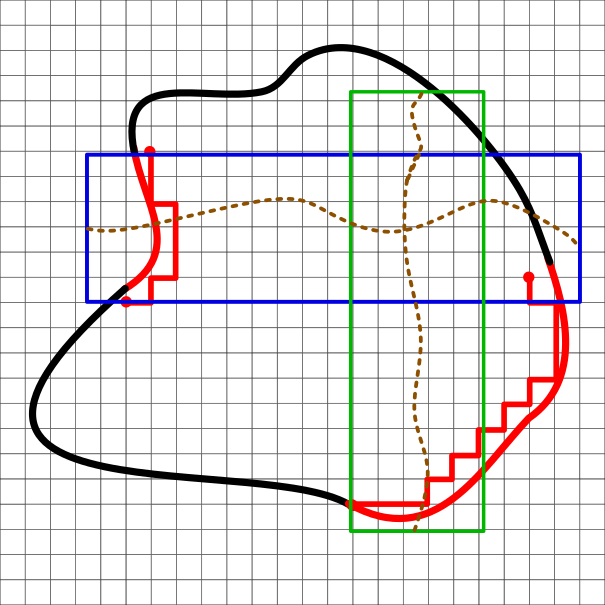
\includegraphics[width=5.0cm]{./RSWpart/omega_2_crossing.png}
\end{figure}
\newpage
    

\section{Individual Research}
\subsection*{Hao: Exponential Decay}
I was intended to study TBD(reference), and in it I found the idea of correlation length and the exponents had to do with the \ref{Course_Progress:Exponentia_Decay} and the exercises. 
The tree exercises I solved were the exponential decay on the size of the connected component $C$ under subcritical stage, correlation length, and Fekete subadditive lemma on $0 \longleftarrow \partial \Lambda_n$.
In solving these exercises, I have more understanding on the relation between different exponents and how can they help us on the study of near critical phenomenon.  
\subsection*{Hsu: Double Phase Transition}
In this section, we introduce the interesting property, double phase transition of $\mathbb{T}_d\times\mathbb{Z}$, which is different from integers lattices $\mathbb{Z}^d$, triangle lattices and regular trees. The number of infinite clusters changes on $[0,1]$; there's no infinite cluster on $(0,p_c)$, infinitely many on $(p_c,p_u)$ and one on $(p_u,1)$, where $p_u$ is defined as \[p_u=\{p\in [0,1] \mid \text{there is a.s. a unique infinite cluster}\}.\]
The property is given by the theorem:
\begin{thm}
For $d\geq 6$, \[0<p_c(\mathbb{T}_d\times\mathbb{Z})<p_u(\mathbb{T}_d\times\mathbb{Z})<1.\]
\end{thm}
For the lower bound of $p_c>0$, we can use the following lemma:
\begin{prop}
For an infinite connected graph $G$, $p_c\geq\frac{1}{\mu}$, where $\mu$ is the connective constant of $G$.
\end{prop}
The main idea is through bounding the $\theta(p)$ by the number of self-avoiding walks of length $n$ with probability $p^n$.\\To make sure $p_c<1$, 
we can use 
\begin{thm}
If $G$ is Cayley graph of a group with exponential growth, then $p_c<1$.
\end{thm}
where we bound the $p_c$ of $G$ by the $p_c$ of its subgraph, lexicographically minimal spanning tree. As for the inequality $p_u<1$, we apply the theorem showed by Babson and Benjamini
\begin{thm}
If $G$ is the Cayley graph of a nonamenable finitely presented group with one end, then $p_u<1$.
\end{thm}
where we consider special graphs and a combinatorial fact to obtain the desired result. The most difficult part is to show the inequality $p_c<p_u$. The essential ingredients are the following:
\begin{thm}
If $G$ is a $d-$regular connected multigraph, then \[\text{cogr}(G)>\sqrt{d-1} \text{ iff } \rho(G)>\frac{2\sqrt{d-1}}{d}\] in which case \[d\rho(G)=\frac{d-1}{\text{cogr}(G)}+\text{cogr}(G).\]
\end{thm}
\begin{cor}
For all $b\geq 1$, we have \[\rho(\mathbb{T}_d\times\mathbb{Z})=\frac{2\sqrt{b}+2}{b+3}.\]
\end{cor}
Of course, the proofs are nontrivial but they give the interesting property that the number of infinite clusters varies on the interval in $p$. \\
\bigskip\\
reference: R. Lyons, Y. Peres, \textit{Probability on Trees and Networks.} (2016)
>>>>>>> ecad8e7a64f7a529bd91aa55c764861710a58540

\section{Future Work}

There are several directions in the future. For example, on the scaling invariant property, RSW theory gave us a way to obtain the uniform probability bounds of crossing events, but we can also ask the question about the scaling limit of a crossing event, not only the uniform bounds. We'll try to apply the discrete analytic ideas developed by Simrnov to extend the scaling problem on different types of lattice.
We can also back to the starting point, thinking the method of finding critical probability or connective constant in some periodic lattice (ex. $\triangle,\ \sixedge,$ etc.) 

\section*{Reference}

\begin{enumerate}
\item S. Smirnov, \textit{Critical percolation in the plane: Conformal invariance, Cardy's formula, scaling limits, C. R. Acad. Sci. Paris} (2001).
\item Hugo Duminil-Copin, \textit{Introduction to Bernoulli percolation}, (2018).
\item Geoffrey R. Grimmett, Ioan Manolescu, \textit{Universality for bond percolation in two dimensions, Ann. Probab.} (2013).
\item R. Lyons, Y. Peres, \textit{Probability on Trees and Networks.} (2016)
\end{enumerate}





\end{document}
